
\subsection{Logistic Regression đa lớp (Softmax Regression) bằng Gradient Descent}

\paragraph{Mô tả ý tưởng.}
Logistic Regression phân loại ảnh MNIST thành 10 lớp chữ số từ
$0$ đến $9$. Mỗi lớp có một vector trọng số, có thể hình dung như
một ``tấm khuôn'' dùng để đánh giá mức độ phù hợp của ảnh với chữ số đó.
Mô hình tính điểm số cho từng lớp, chuyển thành xác suất bằng Softmax,
sau đó chọn lớp có xác suất cao nhất. Các trọng số được học bằng
Mini-batch Gradient Descent nhằm giảm hàm mất mát.

\paragraph{Công thức chính và mã giả.}
Với $X\in\mathbb{R}^{n\times784}$,
$W\in\mathbb{R}^{784\times10}$ và $b\in\mathbb{R}^{10}$,
điểm số và xác suất dự đoán được tính bởi:
\[
Z=XW+b,\qquad
P_{ik}=\frac{e^{Z_{ik}}}{\sum_{j=1}^{10}e^{Z_{ij}}}.
\]
Hàm mất mát Cross-Entropy kết hợp điều chuẩn $L_2$:
\[
\mathcal{L}=-\frac{1}{n}\sum_{i=1}^{n}
\log(P_{i,y_i}+\varepsilon)
+\frac{\lambda}{2}\|W\|_F^2.
\]
Với mini-batch gồm $B$ mẫu, gradient và quy tắc cập nhật là:
\[
G=\frac{P-Y}{B},\qquad
\nabla_W=X^\top G+\lambda W,\qquad
\nabla_b=\sum_{i=1}^{B}G_i,
\]
\[
W\leftarrow W-\eta\nabla_W,\qquad
b\leftarrow b-\eta\nabla_b.
\]
Trong đó, $Y$ là nhãn One-hot, $\eta$ là tốc độ học và
$\lambda$ là hệ số điều chuẩn. Nhãn dự đoán:
$\hat y_i=\arg\max_k P_{ik}$.

\begin{algorithm}[H]
\caption{Huấn luyện và dự đoán Logistic Regression}
\label{alg:logistic}
\begin{algorithmic}[1]
\Function{Fit}{$X,y,\lambda,\eta,E,B$}
    \State Khởi tạo $W$ ngẫu nhiên nhỏ, $b\gets 0$
    \For{$e=1,\ldots,E$}
        \State Xáo trộn dữ liệu và chia thành mini-batch
        \For{mỗi mini-batch $(X_I,Y_I)$}
            \State $P\gets\operatorname{Softmax}(X_IW+b)$
            \State $G\gets(P-Y_I)/B$
            \State $\nabla_W\gets X_I^\top G+\lambda W$
            \State $\nabla_b\gets\sum_i G_i$
            \State $W\gets W-\eta\nabla_W$
            \State $b\gets b-\eta\nabla_b$
        \EndFor
        \State Ghi nhận train loss và validation accuracy
    \EndFor
    \State \Return $W,b$
\EndFunction
\Function{Predict}{$X,W,b$}
    \State $P\gets\operatorname{Softmax}(XW+b)$
    \State \Return $\arg\max_k P_{ik}$ với mỗi ảnh $i$
\EndFunction
\end{algorithmic}
\end{algorithm}

\paragraph{Chi tiết cài đặt.}
Mô hình được xây dựng bằng Python và NumPy. Hàm
\texttt{fit()} huấn luyện theo mini-batch; \texttt{predict\_proba()}
trả về xác suất 10 lớp và \texttt{predict()} chọn lớp dự đoán.
Khi tính Softmax, trừ giá trị lớn nhất mỗi hàng trước khi lấy hàm mũ
để hạn chế tràn số. Các siêu tham số gồm \texttt{lr}, \texttt{lam},
\texttt{epochs}, \texttt{batch\_size} và \texttt{seed}.

\paragraph{Cách kiểm chứng.}
\begin{enumerate}
    \item \textbf{Tính toán thủ công.}
    Với ví dụ minh họa ba lớp có $\mathbf z=[1,2,0.5]$,
    Softmax cho $\mathbf P\approx[0.2312,0.6285,0.1403]$.
    Tổng xác suất xấp xỉ $1$, lớp dự đoán là lớp $2$.
    Nếu nhãn đúng là lớp $2$, Cross-Entropy xấp xỉ
    $-\ln(0.6285)=0.4648$. MNIST thực tế sử dụng 10 lớp.

    \item \textbf{Kiểm tra gradient.}
    Trên 20 ảnh, với $\lambda=10^{-3}$, seed $=0$ và
    $\epsilon=10^{-5}$, sai số tương đối lớn nhất trên 10
    trọng số được kiểm tra là $4.90\times10^{-7}<10^{-6}$,
    đạt ngưỡng kiểm tra gradient theo trọng số.

    \item \textbf{Kiểm tra huấn luyện.}
    Sau 20 epoch, train loss giảm từ khoảng $0.408$ xuống
    $0.277$; validation accuracy đạt khoảng $91.65\%$
    tại epoch $19$. Mô hình có xu hướng hội tụ; kết quả
    được minh họa ở Hình~\ref{fig:logistic-training}.

    \item \textbf{Đối chiếu với scikit-learn.}
    So sánh với \texttt{LogisticRegression} của scikit-learn
    trên cùng dữ liệu và cách tiền xử lý; dùng accuracy để
    đánh giá mức độ tương đồng giữa hai mô hình. (Bảng~\ref{tab:sklearn}).
\end{enumerate}

\begin{figure}[H]
    \centering
    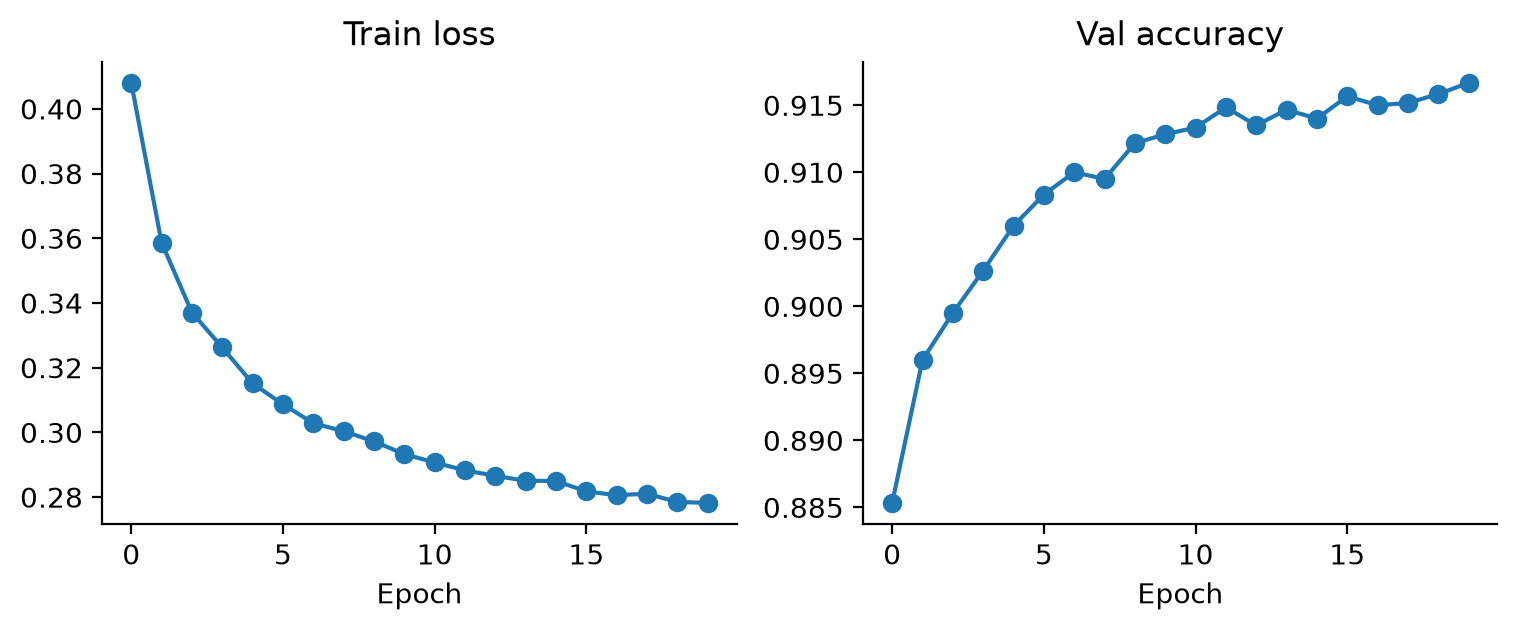
\includegraphics[width=0.72\linewidth]{figures/lr_curve.png}
    \caption{Train loss và validation accuracy của Logistic
    Regression trên MNIST.}
    \label{fig:logistic-training}
\end{figure}
